\documentclass[11pt,a4paper]{article}

% ---------------------------------------------------------------- packages --
\usepackage[utf8]{inputenc}
\usepackage[T1]{fontenc}
\usepackage[margin=1in]{geometry}
\usepackage{amsmath,amssymb}
\usepackage{graphicx}
\usepackage{booktabs}
\usepackage{longtable}
\usepackage{array}
\usepackage{listings}
\usepackage{xcolor}
\usepackage{caption}
\usepackage[hidelinks]{hyperref}

\graphicspath{{../../docs/mindmaps/}{../../docs/screenshots/}}

% ------------------------------------------------------------- listing style -
\definecolor{codegray}{gray}{0.95}
\definecolor{codegreen}{rgb}{0.0,0.5,0.0}
\definecolor{codeblue}{rgb}{0.1,0.1,0.6}
\lstdefinestyle{pseudo}{
  basicstyle=\ttfamily\small,
  backgroundcolor=\color{codegray},
  frame=single, framerule=0pt, breaklines=true,
  columns=fullflexible, keepspaces=true,
  xleftmargin=6pt, xrightmargin=6pt, aboveskip=6pt, belowskip=6pt,
}
\lstdefinestyle{py}{
  language=Python, style=pseudo,
  keywordstyle=\color{codeblue}\bfseries,
  commentstyle=\color{codegreen}\itshape,
  stringstyle=\color{purple},
  numbers=left, numberstyle=\tiny\color{gray}, numbersep=6pt,
}

\newcolumntype{L}[1]{>{\raggedright\arraybackslash}p{#1}}

% ----------------------------------------------------------------- metadata --
\title{\textbf{SOEN 6011 --- Deliverable 2}\\[2pt]
       \large Function F6: The Real Beta Function $B(x,y)$\\
       From-Scratch Implementation, Tkinter GUI, Repository, and Updated Requirements}
\author{Shoban Bhowmik \quad (Student ID 40325778)}
\date{2026-07-24 \quad (version 0.2.0)}

\begin{document}
\maketitle

\begin{abstract}
\noindent This report documents Deliverable~2 for Function~F6, the real Beta
function $B(x,y)=\Gamma(x)\Gamma(y)/\Gamma(x+y)$ scoped to $x>0,\,y>0$.
Problem~5 reimplements the function \emph{from scratch}: the three elementary
primitives the Deliverable~1 prototype borrowed from Python's \texttt{math}
module ($\ln$, $\exp$, $\sin$, and the constant $\pi$) are rebuilt using only
arithmetic and control flow, via range reduction and convergent series, and the
result is wrapped in a Tkinter graphical interface with a typed exception
hierarchy and helpful error messages. Problem~6 places the source in a public
Git repository with an incremental, high-quality commit history and a README.
Problem~7 evolves the requirements baseline from v0.1 to v0.2 on the basis of the
implemented behaviour. Every problem was supported by a documented CASTROFF
generative-AI prompt whose output was critically evaluated and independently
verified. A re-runnable harness passes \textbf{27/27} checks; the from-scratch
build reproduces the D1 accuracy \emph{exactly}, with a worst-case relative error
of $1.17\times10^{-14}$, eight orders of magnitude inside the $10^{-6}$ tolerance.
\end{abstract}

\tableofcontents
\bigskip

% ============================================================================
\section{Introduction and scope}
Deliverable~2 modifies the Deliverable~1 prototype rather than starting over
(the project is iterative and incremental). D1 selected \textbf{Algorithm~B} ---
the Gamma identity $B(x,y)=\Gamma(x)\Gamma(y)/\Gamma(x+y)$ evaluated in the log
domain, $B=\exp(\ln\Gamma(x)+\ln\Gamma(y)-\ln\Gamma(x+y))$, with a hand-written
Lanczos $\ln\Gamma$~\cite{lanczos1964gamma,press2007numerical} --- and shipped a
command-line prototype (\texttt{src/cli.py}) that borrowed only four elementary
primitives from \texttt{math}. This deliverable removes that dependency
(Problem~5), adds a Tkinter GUI (Problem~5), publishes the code (Problem~6), and
updates the requirements (Problem~7). The supported domain remains $x>0,\,y>0$
(decision~D-001); reference definitions are from the NIST DLMF~\cite{dlmf512} and
Abramowitz~\&~Stegun~\cite{abramowitz1964handbook}.

% ============================================================================
\section{Problem 5 --- From-scratch implementation and GUI}
\label{sec:p5}

\subsection{Freezing the ``from scratch'' boundary}
The Problem~5 rule exempts \emph{input, output, arithmetic, and user-interface}
facilities and prohibits every other built-in or library function. The
dependency inventory of the D1 prototype identified exactly four mathematical
borrowings; Table~\ref{tab:boundary} classifies them and names their from-scratch
replacements (decision~D-008). No \texttt{math.gamma}, \texttt{math.lgamma}, or
library \texttt{beta} was ever used --- those would defeat the exercise.

\begin{table}[htbp]\centering\small
\caption{From-scratch boundary: prohibited primitives and their replacements.}
\label{tab:boundary}
\begin{tabular}{@{}L{2.4cm} L{4.4cm} L{6.4cm}@{}}
\toprule
\textbf{Borrowed (D1)} & \textbf{Role} & \textbf{D2 replacement (\texttt{elementary.py})}\\
\midrule
\texttt{math.log} & natural logarithm & \texttt{ln} --- mantissa reduction $x=m\cdot2^{e}$ + atanh series\\
\texttt{math.exp} & exponential & \texttt{exp} --- reduction $x=k\ln2+r$ + Taylor series\\
\texttt{math.sin} & reflection only & \texttt{sin} --- argument reduction + Taylor series\\
\texttt{math.pi} & constant $\pi$ & \texttt{PI} --- correctly-rounded double literal\\
\texttt{math.isfinite} & overflow guard & \texttt{is\_finite} --- IEEE comparison (not maths)\\
\bottomrule
\end{tabular}
\end{table}

Retained facilities are arithmetic operators, the \texttt{int}/\texttt{float}
casts (numeric conversion/parsing), string formatting (output), Tkinter (UI), and
exceptions (explicitly required). The harness check \textbf{IMPL-01} scans every
shipped module and fails if any imports \texttt{math}, \texttt{numpy},
\texttt{scipy}, \texttt{mpmath}, or \texttt{cmath}; it passes.

\subsection{The elementary functions}
Each primitive follows the standard recipe used by production math
libraries~\cite{muller2016elementary,cody1980software}: \emph{range reduction} to
a small interval, a \emph{rapidly convergent series}, then \emph{reconstruction}.
Every loop terminates in a bounded number of steps (REL-03): the series stop when
the next term falls below the working precision, and the power-of-two scaling
exits as soon as the magnitude leaves the double range. The logarithm is
representative:

\begin{lstlisting}[style=py]
def ln(x):
    if x <= 0.0:
        raise ValueError("ln is defined only for x > 0")
    e = 0; m = x                      # reduce mantissa into [1/sqrt2, sqrt2)
    while m >= _SQRT2:   m *= 0.5; e += 1
    while m < _SQRT1_2:  m *= 2.0; e -= 1
    s = (m - 1.0) / (m + 1.0)         # |s| <= 0.1716 -> fast series
    s2 = s * s; term = s; total = s; denom = 1
    while True:                        # ln(m) = 2*(s + s^3/3 + s^5/5 + ...)
        term *= s2; denom += 2
        delta = term / denom; total += delta
        if abs(delta) < _EPS * abs(total) + _EPS:
            break
    return e * LN2 + 2.0 * total       # ln(x) = e*ln2 + ln(m)
\end{lstlisting}

\noindent Verified against a trusted oracle over wide ranges, the primitives
reach machine precision: worst relative error $\le 6\times10^{-15}$ for $\exp$,
$\le 6\times10^{-16}$ for $\ln$, and worst absolute error $\le 9\times10^{-16}$
for $\sin$ (harness check ACC-03p). Full derivations and pseudocode for all three
are in \texttt{docs/algorithms/elementary\_functions.md}.

\subsection{Architecture and exception handling}
The source is separated so the numerical core is testable without a GUI and
reusable by both front-ends: \texttt{elementary.py} (primitives) $\rightarrow$
\texttt{beta\_core.py} (pure $\ln\Gamma$/$\beta$, imports only
\texttt{elementary}) $\rightarrow$ \texttt{validation.py} (parsing + messages)
and \texttt{gui.py} (Tkinter). Errors use a typed hierarchy
(decision~D-011): a base \texttt{BetaError} with \texttt{InputError}
(\texttt{Empty}/\texttt{NonNumeric}/\texttt{NonFinite}), \texttt{DomainError},
\texttt{RangeError}, and \texttt{NumericalError}
(\texttt{NumericalRange}/\texttt{Convergence}) subclasses, each carrying a
user-facing message. This lets the GUI catch input errors and numerical errors
separately (ERR-02) while a single \texttt{except BetaError} still guarantees no
traceback reaches the user (REL-01). The core signals overflow explicitly:

\begin{lstlisting}[style=py]
def beta(x, y):
    if x <= DOMAIN_MIN or y <= DOMAIN_MIN:
        raise DomainError("... supported for x > 0 and y > 0 ...")
    result = el.exp(beta_ln(x, y))             # log domain avoids overflow
    if not el.is_finite(result):
        raise NumericalRangeError("... too large or too small ...")
    return result
\end{lstlisting}

\subsection{The Tkinter GUI}
The interface was wireframed before coding (decision~D-010,
\texttt{docs/gui\_wireframe.md}) and traces to the persona ``Maya Fernandes'': a
single resizable window with two labelled fields that state the domain at the
point of input (``\texttt{x (must be > 0)}''), \textsf{Calculate}/\textsf{Clear}/
\textsf{Help} buttons, and one status line. It is keyboard-first (UI-01): initial
focus on $x$; Tab order $x\to y\to$ Calculate $\to$ Clear; \textsf{Enter}
computes; \textsf{Escape} clears; \textsf{F1} opens Help. Status meaning is
carried by a leading word and a glyph, with colour only as a redundant cue
(ACC-03). Figures~\ref{fig:guivalid}--\ref{fig:guierr} show a valid computation
and an out-of-domain error; each expected failure produces a specific message,
never a traceback (REL-01, ERR-01).

\begin{figure}[htbp]
  \centering
  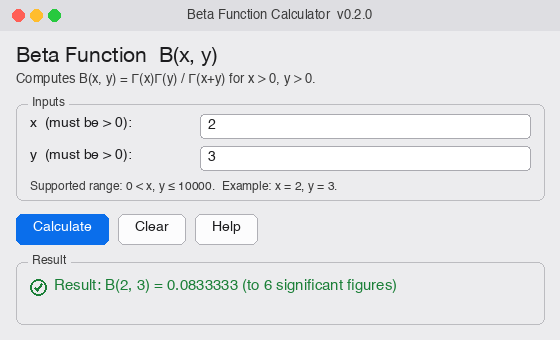
\includegraphics[width=0.72\textwidth]{gui_valid.png}
  \caption{Valid case $B(2,3)=0.0833333$ (=1/12), shown to six significant figures.}
  \label{fig:guivalid}
\end{figure}
\begin{figure}[htbp]
  \centering
  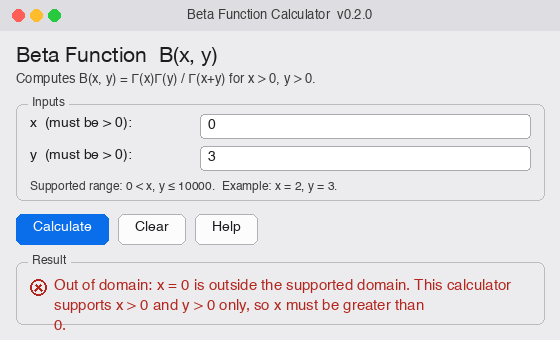
\includegraphics[width=0.72\textwidth]{gui_domain.png}
  \caption{Out-of-domain input ($x=0$): a specific, corrective message
           (ERR-01), conveyed as text and not by colour alone (ACC-03).}
  \label{fig:guierr}
\end{figure}

\noindent\emph{Note on figures.} A live screen grab of a Tk window is blocked in
a headless session, so Figures~\ref{fig:guivalid}--\ref{fig:guierr} are layout
renders that reproduce the exact widgets and status strings emitted by
\texttt{src/gui.py} (verified in \texttt{tests/verify\_d2.py}, checks
GUI-01--GUI-06); the genuine window is shown in the live Zoom demonstration.

\subsection{Verification}
\label{sec:verify}
The re-runnable harness \texttt{tests/verify\_d2.py} passes \textbf{27/27}
checks. It confirms the no-library boundary (IMPL-01); the primitive accuracy
against \texttt{math} used \emph{only as an oracle} (ACC-03p); the Beta accuracy
across all 18 trusted reference values with a worst relative error of
$1.17\times10^{-14}$ including the $B(0.2,0.3)$ corner (ACC-01); symmetry; the
five validation paths each raising their specific typed exception with a helpful
message (VAL/ERR); no non-finite output over 36 large/small inputs (REL-02);
bounded work (REL-03); $7.8\times10^{-3}$\,ms per computation (PERF-01); a
subprocess GUI launch (POR-01); and the six GUI event-handler behaviours. The
requirement-by-requirement matrix is in
\texttt{docs/verification\_matrix\_d2.md}.

\subsection{GAI use and critical evaluation (Problem 5)}
\textbf{Tool:} Claude (Opus~4.8) via Claude Code. \textbf{Prompt type:}
generative + transformational (refactor to from-scratch) with GUI design. The
CASTROFF prompt supplied \texttt{src/cli.py} and the borrowed-primitive list, and
required (i)~a frozen boundary, (ii)~from-scratch $\ln$/$\exp$/$\sin$/$\pi$ via
range reduction + series while keeping the Lanczos $\ln\Gamma$, and (iii)~a
wireframed Tkinter GUI over a pure core with a typed exception hierarchy.
\textbf{Accepted:} the reduction-plus-series design, the \texttt{BetaError}
hierarchy, and the compute/UI separation. \textbf{Verified independently:} rather
than trusting the output, the harness confirmed the shipped modules import no
math library and that the primitives match \texttt{math} to $\le6\times10^{-15}$
and the Beta core reproduces the D1 accuracy exactly. \textbf{Adjusted:} floor/
round/finiteness were implemented by hand and $2^{k}$ by bounded repeated
multiplication, so the boundary is honest. \textbf{Rejected:} any use of
\texttt{math}/\texttt{numpy}, CORDIC/minimax (unnecessary complexity, D-009), and
colour-only status (ACC-03).

% ============================================================================
\section{Problem 6 --- Repository, commits, and README}
\label{sec:p6}
The source is under Git with an \emph{incremental} history (decision~D-013): one
cohesive change per commit, with imperative, specific subjects (e.g.\ ``Add
from-scratch elementary functions (ln, exp, sin)'', ``Add Tkinter GUI over the
pure core''), separating scaffold, primitives, core, validation/exceptions, GUI,
tests, and documentation rather than a single bulk upload, so the commit log shows
how the project evolved. A \texttt{.gitignore} excludes byte-code, \texttt{.DS\_Store},
LaTeX build artefacts, IDE settings, and submission zips. The \texttt{README.md}
lets a fresh user run the program: purpose and definition, prerequisites, the
exact command (\texttt{python3 src/gui.py}), usage examples with screenshots, an
error/troubleshooting guide, the repository structure, the version, and
attribution. The public host uses the author's own account; the repository URL is
\texttt{<PUBLIC-REPO-URL>} and is recorded in the README on publication. Commit
subjects and the publish commands are listed in the README and the D2 execution
steps.

% ============================================================================
\section{Problem 7 --- Updated requirements (v0.1 $\rightarrow$ v0.2)}
\label{sec:p7}
The requirements were compared line-by-line with the actual D2 behaviour and
re-frozen as baseline~\textbf{v0.2} (decision~D-012). All v0.1 identifiers were
retained for traceability; three requirements were added and several reworded for
the GUI. Table~\ref{tab:changes} is the change log; the full v0.2 table (24
requirements) is in \texttt{docs/requirements/requirements\_updated\_v0.2.md}.

\begin{table}[htbp]\centering\small
\caption{Requirement changes v0.1 $\rightarrow$ v0.2 (all changes discovered
through implementation unless noted).}
\label{tab:changes}
\begin{tabular}{@{}L{2.6cm} L{10.4cm}@{}}
\toprule
\textbf{Requirement} & \textbf{Change and reason}\\
\midrule
FR-01/03/04/05, USE-01/02 & CLI prompts/commands $\rightarrow$ GUI labels/affordances (UI moved to Tkinter).\\
VAL-02 & now also rejects non-finite text (\texttt{inf}/\texttt{nan}), which \texttt{float()} would otherwise accept.\\
ACC-01, A-05 & re-scoped to the from-scratch build and re-validated (worst rel.\ err.\ unchanged at $1.17\times10^{-14}$).\\
ACC-03 & priority S~$\rightarrow$~M --- accessibility is first-class for the GUI (design decision).\\
REL-01 & strengthened: no traceback may reach the GUI; expected failures caught as typed \texttt{BetaError}s.\\
REL-02 & now raises an explicit \texttt{NumericalRangeError} instead of a silent guard.\\
POR-01 & entry point \texttt{src/cli.py} $\rightarrow$ \texttt{src/gui.py}.\\
\textbf{IMPL-01} (new) & the mathematics must be from scratch (Problem~5 mandate, D-008).\\
\textbf{UI-01} (new) & the GUI must be fully keyboard-operable.\\
\textbf{ERR-02} (new) & distinct exception types for input vs numerical errors.\\
\bottomrule
\end{tabular}
\end{table}

\noindent No requirement was deleted; superseded wording is preserved in v0.1.
Assumptions A-04 (magnitude cap) and A-05 (tolerance) --- flagged in D1 for
re-validation --- were confirmed against the from-scratch build, and A-07 was
added for the elementary-function accuracy.

\paragraph{GAI use (Problems 6--7).} \textbf{Tool:} Claude (Opus~4.8).
For Problem~6 the CASTROFF prompt (advisory) produced the \texttt{.gitignore}, the
incremental commit plan, and the README; the \emph{publish} step was deliberately
left to the author's own account (an outward-facing action), with exact commands
provided. For Problem~7 the CASTROFF prompt (transformational + review) evolved
the v0.1 baseline; every change was checked against a verification-matrix entry
and a decision-log rationale, and superseded wording was preserved rather than
deleted. Full logs: \texttt{docs/prompts/gai\_prompt\_log.md}.

% ============================================================================
\section{Known limitations (honest disclosure)}
The domain is $x,y>0$ only (no analytic continuation or complex arguments);
magnitudes above $10^{4}$ are rejected by design; very large near-equal inputs
(e.g.\ $B(10^{4},10^{4})$) correctly underflow to the finite double $0.0$;
accuracy is bounded by the Lanczos $g{=}7$ set ($\approx15$ digits) and the
series precision (verified $\le6\times10^{-15}$); and the GUI figures are renders,
with the live window shown in the demo. Each is a documented scope boundary or
assumption (D-001/D-004/D-007/D-008, A-01/A-04/A-05/A-06), not a correctness
defect within the supported domain.

% ============================================================================
\section{Decision rationale summary}
D-008 freezes the from-scratch boundary; D-009 chooses range-reduction-plus-series
for the primitives; D-010 fixes the wireframed GUI; D-011 defines the typed
exception hierarchy; D-012 freezes requirements~v0.2; D-013 sets the public-repo
and commit strategy. All are recorded in
\texttt{docs/decisions/decision\_log.md}, and every GAI interaction is logged with
its prompt, output summary, critical evaluation, and independent verification in
\texttt{docs/prompts/gai\_prompt\_log.md}.

% ----------------------------------------------------------------- references
\bibliographystyle{ieeetr}
\bibliography{references}

\end{document}
